% Options for packages loaded elsewhere
\PassOptionsToPackage{unicode}{hyperref}
\PassOptionsToPackage{hyphens}{url}
\PassOptionsToPackage{dvipsnames,svgnames,x11names}{xcolor}
%
\documentclass[
  letterpaper,
  DIV=11,
  numbers=noendperiod]{scrartcl}

\usepackage{amsmath,amssymb}
\usepackage{lmodern}
\usepackage{iftex}
\ifPDFTeX
  \usepackage[T1]{fontenc}
  \usepackage[utf8]{inputenc}
  \usepackage{textcomp} % provide euro and other symbols
\else % if luatex or xetex
  \usepackage{unicode-math}
  \defaultfontfeatures{Scale=MatchLowercase}
  \defaultfontfeatures[\rmfamily]{Ligatures=TeX,Scale=1}
\fi
% Use upquote if available, for straight quotes in verbatim environments
\IfFileExists{upquote.sty}{\usepackage{upquote}}{}
\IfFileExists{microtype.sty}{% use microtype if available
  \usepackage[]{microtype}
  \UseMicrotypeSet[protrusion]{basicmath} % disable protrusion for tt fonts
}{}
\makeatletter
\@ifundefined{KOMAClassName}{% if non-KOMA class
  \IfFileExists{parskip.sty}{%
    \usepackage{parskip}
  }{% else
    \setlength{\parindent}{0pt}
    \setlength{\parskip}{6pt plus 2pt minus 1pt}}
}{% if KOMA class
  \KOMAoptions{parskip=half}}
\makeatother
\usepackage{xcolor}
\setlength{\emergencystretch}{3em} % prevent overfull lines
\setcounter{secnumdepth}{-\maxdimen} % remove section numbering
% Make \paragraph and \subparagraph free-standing
\ifx\paragraph\undefined\else
  \let\oldparagraph\paragraph
  \renewcommand{\paragraph}[1]{\oldparagraph{#1}\mbox{}}
\fi
\ifx\subparagraph\undefined\else
  \let\oldsubparagraph\subparagraph
  \renewcommand{\subparagraph}[1]{\oldsubparagraph{#1}\mbox{}}
\fi


\providecommand{\tightlist}{%
  \setlength{\itemsep}{0pt}\setlength{\parskip}{0pt}}\usepackage{longtable,booktabs,array}
\usepackage{calc} % for calculating minipage widths
% Correct order of tables after \paragraph or \subparagraph
\usepackage{etoolbox}
\makeatletter
\patchcmd\longtable{\par}{\if@noskipsec\mbox{}\fi\par}{}{}
\makeatother
% Allow footnotes in longtable head/foot
\IfFileExists{footnotehyper.sty}{\usepackage{footnotehyper}}{\usepackage{footnote}}
\makesavenoteenv{longtable}
\usepackage{graphicx}
\makeatletter
\def\maxwidth{\ifdim\Gin@nat@width>\linewidth\linewidth\else\Gin@nat@width\fi}
\def\maxheight{\ifdim\Gin@nat@height>\textheight\textheight\else\Gin@nat@height\fi}
\makeatother
% Scale images if necessary, so that they will not overflow the page
% margins by default, and it is still possible to overwrite the defaults
% using explicit options in \includegraphics[width, height, ...]{}
\setkeys{Gin}{width=\maxwidth,height=\maxheight,keepaspectratio}
% Set default figure placement to htbp
\makeatletter
\def\fps@figure{htbp}
\makeatother

\KOMAoption{captions}{tableheading}
\makeatletter
\makeatother
\makeatletter
\makeatother
\makeatletter
\@ifpackageloaded{caption}{}{\usepackage{caption}}
\AtBeginDocument{%
\ifdefined\contentsname
  \renewcommand*\contentsname{Table of contents}
\else
  \newcommand\contentsname{Table of contents}
\fi
\ifdefined\listfigurename
  \renewcommand*\listfigurename{List of Figures}
\else
  \newcommand\listfigurename{List of Figures}
\fi
\ifdefined\listtablename
  \renewcommand*\listtablename{List of Tables}
\else
  \newcommand\listtablename{List of Tables}
\fi
\ifdefined\figurename
  \renewcommand*\figurename{Figure}
\else
  \newcommand\figurename{Figure}
\fi
\ifdefined\tablename
  \renewcommand*\tablename{Table}
\else
  \newcommand\tablename{Table}
\fi
}
\@ifpackageloaded{float}{}{\usepackage{float}}
\floatstyle{ruled}
\@ifundefined{c@chapter}{\newfloat{codelisting}{h}{lop}}{\newfloat{codelisting}{h}{lop}[chapter]}
\floatname{codelisting}{Listing}
\newcommand*\listoflistings{\listof{codelisting}{List of Listings}}
\makeatother
\makeatletter
\@ifpackageloaded{caption}{}{\usepackage{caption}}
\@ifpackageloaded{subcaption}{}{\usepackage{subcaption}}
\makeatother
\makeatletter
\@ifpackageloaded{tcolorbox}{}{\usepackage[many]{tcolorbox}}
\makeatother
\makeatletter
\@ifundefined{shadecolor}{\definecolor{shadecolor}{rgb}{.97, .97, .97}}
\makeatother
\makeatletter
\makeatother
\ifLuaTeX
  \usepackage{selnolig}  % disable illegal ligatures
\fi
\IfFileExists{bookmark.sty}{\usepackage{bookmark}}{\usepackage{hyperref}}
\IfFileExists{xurl.sty}{\usepackage{xurl}}{} % add URL line breaks if available
\urlstyle{same} % disable monospaced font for URLs
\hypersetup{
  pdftitle={Protección de semillas},
  colorlinks=true,
  linkcolor={blue},
  filecolor={Maroon},
  citecolor={Blue},
  urlcolor={Blue},
  pdfcreator={LaTeX via pandoc}}

\title{Protección de semillas}
\author{}
\date{}

\begin{document}
\maketitle
\ifdefined\Shaded\renewenvironment{Shaded}{\begin{tcolorbox}[boxrule=0pt, interior hidden, frame hidden, borderline west={3pt}{0pt}{shadecolor}, sharp corners, enhanced, breakable]}{\end{tcolorbox}}\fi

\hypertarget{dataset}{%
\subsection{Dataset}\label{dataset}}

\begin{longtable}[]{@{}llrrr@{}}
\toprule()
cultivo & prod & MDP & Tandil & La Dulce \\
\midrule()
\endhead
Cebada & CHECK & 6 & 3 & NA \\
Cebada & CURACYT & 3 & 3 & NA \\
Cebada & RANCONA\_TRIO\_400 & 3 & 3 & 3 \\
Cebada & RIZODERMA\_SX & 3 & 3 & 3 \\
Cebada & RIZODERMA\_SX + VITAGROW + STZN & 3 & 3 & 3 \\
Cebada & SISTIVA\_PREMIS & 3 & 3 & 3 \\
Cebada & SISTIVA\_PREMIS + ALZ\_12051 & 3 & 3 & 3 \\
Cebada & SISTIVA\_PREMIS\_2X & 3 & 3 & NA \\
Cebada & VIBRANCE\_INTEGRAL & 3 & 3 & 3 \\
Trigo & CHECK & 3 & 3 & NA \\
Trigo & CURACYT & 3 & 3 & NA \\
Trigo & RANCONA\_TRIO\_300 & 3 & 3 & 3 \\
Trigo & RIZODERMA & 3 & 3 & 3 \\
Trigo & RIZODERMA + VITAGROW + STZN & 3 & 3 & 3 \\
Trigo & SISTIVA\_PREMIS & 3 & 3 & 3 \\
Trigo & SISTIVA\_PREMIS + ALLTEC\_ZN & 3 & 3 & NA \\
Trigo & SISTIVA\_PREMIS + ALZ\_12051 & 3 & 3 & 3 \\
Trigo & SISTIVA\_PREMIS\_2X & 3 & NA & NA \\
Trigo & VIBRANCE\_INTEGRAL & 3 & 3 & 3 \\
\bottomrule()
\end{longtable}

\hypertarget{cobertura}{%
\section{Cobertura}\label{cobertura}}

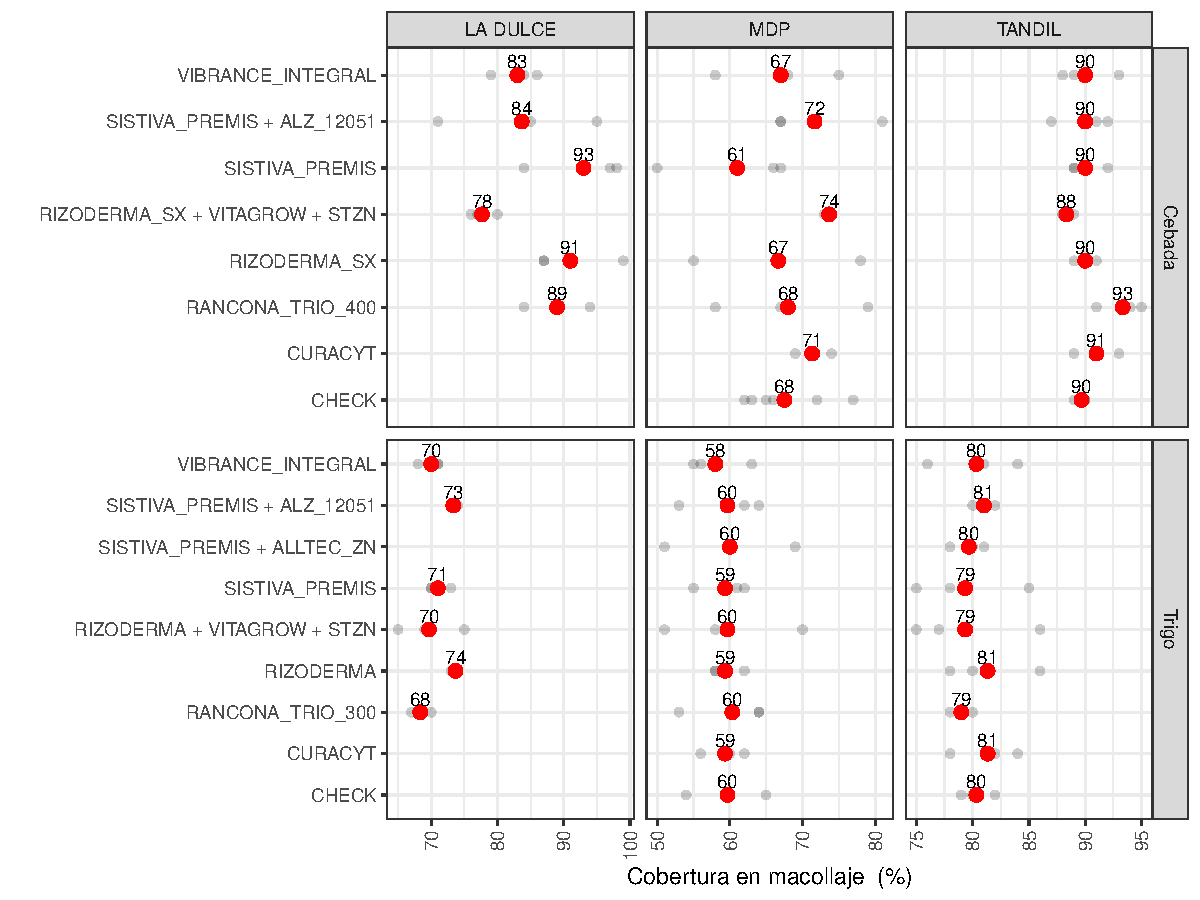
\includegraphics{curasem_files/figure-pdf/cober_plot-1.pdf}

\hypertarget{cebada}{%
\subsection{Cebada}\label{cebada}}

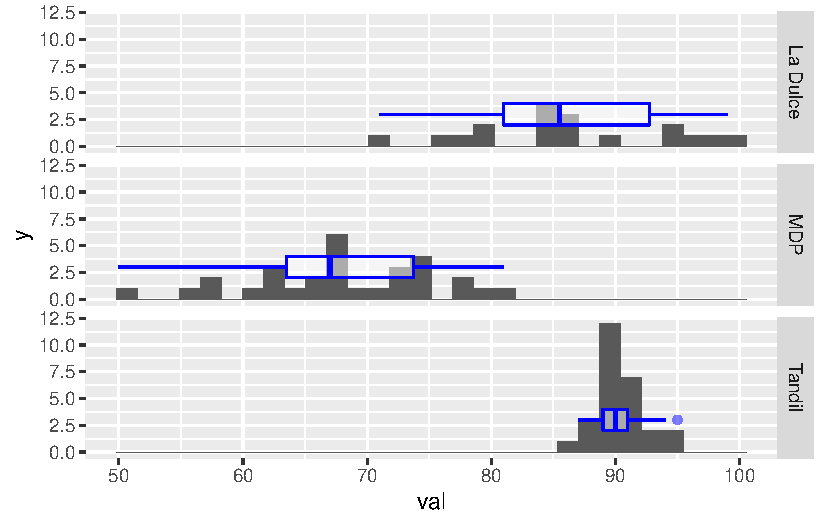
\includegraphics{curasem_files/figure-pdf/unnamed-chunk-7-1.pdf}

\hypertarget{anuxe1lisis-conjunto-de-6-tratamientos}{%
\subsubsection{Análisis conjunto de 6
tratamientos}\label{anuxe1lisis-conjunto-de-6-tratamientos}}

\begin{verbatim}
                                       sitio La Dulce MDP Tandil
cultivo prod                                                    
Cebada  RANCONA_TRIO_400                            3   3      3
        RIZODERMA_SX                                3   3      3
        RIZODERMA_SX + VITAGROW + STZN              3   3      3
        SISTIVA_PREMIS                              3   3      3
        SISTIVA_PREMIS + ALZ_12051                  3   3      3
        VIBRANCE_INTEGRAL                           3   3      3
\end{verbatim}

\begin{longtable}[]{@{}lrrr@{}}
\toprule()
& Chisq & Df & Pr(\textgreater Chisq) \\
\midrule()
\endhead
prod & 3.098456 & 5 & 0.6848099 \\
\bottomrule()
\end{longtable}

\begin{longtable}[]{@{}
  >{\raggedright\arraybackslash}p{(\columnwidth - 14\tabcolsep) * \real{0.0349}}
  >{\raggedright\arraybackslash}p{(\columnwidth - 14\tabcolsep) * \real{0.3605}}
  >{\raggedleft\arraybackslash}p{(\columnwidth - 14\tabcolsep) * \real{0.1047}}
  >{\raggedleft\arraybackslash}p{(\columnwidth - 14\tabcolsep) * \real{0.1047}}
  >{\raggedleft\arraybackslash}p{(\columnwidth - 14\tabcolsep) * \real{0.1047}}
  >{\raggedleft\arraybackslash}p{(\columnwidth - 14\tabcolsep) * \real{0.1047}}
  >{\raggedleft\arraybackslash}p{(\columnwidth - 14\tabcolsep) * \real{0.1047}}
  >{\raggedright\arraybackslash}p{(\columnwidth - 14\tabcolsep) * \real{0.0814}}@{}}
\toprule()
\begin{minipage}[b]{\linewidth}\raggedright
\end{minipage} & \begin{minipage}[b]{\linewidth}\raggedright
prod
\end{minipage} & \begin{minipage}[b]{\linewidth}\raggedleft
response
\end{minipage} & \begin{minipage}[b]{\linewidth}\raggedleft
SE
\end{minipage} & \begin{minipage}[b]{\linewidth}\raggedleft
df
\end{minipage} & \begin{minipage}[b]{\linewidth}\raggedleft
lower.CL
\end{minipage} & \begin{minipage}[b]{\linewidth}\raggedleft
upper.CL
\end{minipage} & \begin{minipage}[b]{\linewidth}\raggedright
.group
\end{minipage} \\
\midrule()
\endhead
3 & RANCONA\_TRIO\_400 & 85.09150 & 6.602184 & 2.486955 & 55.63074 &
99.59272 & a \\
6 & RIZODERMA\_SX & 84.53233 & 6.702726 & 2.486955 & 54.85602 & 99.48747
& a \\
5 & SISTIVA\_PREMIS & 83.94616 & 6.804832 & 2.486955 & 54.05485 &
99.36620 & a \\
4 & SISTIVA\_PREMIS + ALZ\_12051 & 82.98157 & 6.965915 & 2.486955 &
52.75955 & 99.14351 & a \\
2 & VIBRANCE\_INTEGRAL & 80.98873 & 7.273533 & 2.486955 & 50.16732 &
98.59961 & a \\
1 & RIZODERMA\_SX + VITAGROW + STZN & 80.30965 & 7.371199 & 2.486955 &
49.30783 & 98.39044 & a \\
\bottomrule()
\end{longtable}

\hypertarget{anuxe1lisis-conjunto-de-mdp-tandil}{%
\subsubsection{Análisis conjunto de MDP +
Tandil}\label{anuxe1lisis-conjunto-de-mdp-tandil}}

\begin{verbatim}
                               sitio MDP Tandil
prod                                           
CHECK                                  6      3
CURACYT                                3      3
RANCONA_TRIO_400                       3      3
RIZODERMA_SX                           3      3
RIZODERMA_SX + VITAGROW + STZN         3      3
SISTIVA_PREMIS                         3      3
SISTIVA_PREMIS + ALZ_12051             3      3
SISTIVA_PREMIS_2X                      3      3
VIBRANCE_INTEGRAL                      3      3
\end{verbatim}

\begin{longtable}[]{@{}lrrr@{}}
\toprule()
& Chisq & Df & Pr(\textgreater Chisq) \\
\midrule()
\endhead
prod & 5.853181 & 8 & 0.6636737 \\
\bottomrule()
\end{longtable}

\begin{longtable}[]{@{}
  >{\raggedright\arraybackslash}p{(\columnwidth - 14\tabcolsep) * \real{0.0349}}
  >{\raggedright\arraybackslash}p{(\columnwidth - 14\tabcolsep) * \real{0.3605}}
  >{\raggedleft\arraybackslash}p{(\columnwidth - 14\tabcolsep) * \real{0.1047}}
  >{\raggedleft\arraybackslash}p{(\columnwidth - 14\tabcolsep) * \real{0.1047}}
  >{\raggedleft\arraybackslash}p{(\columnwidth - 14\tabcolsep) * \real{0.1047}}
  >{\raggedleft\arraybackslash}p{(\columnwidth - 14\tabcolsep) * \real{0.1047}}
  >{\raggedleft\arraybackslash}p{(\columnwidth - 14\tabcolsep) * \real{0.1047}}
  >{\raggedright\arraybackslash}p{(\columnwidth - 14\tabcolsep) * \real{0.0814}}@{}}
\toprule()
\begin{minipage}[b]{\linewidth}\raggedright
\end{minipage} & \begin{minipage}[b]{\linewidth}\raggedright
prod
\end{minipage} & \begin{minipage}[b]{\linewidth}\raggedleft
response
\end{minipage} & \begin{minipage}[b]{\linewidth}\raggedleft
SE
\end{minipage} & \begin{minipage}[b]{\linewidth}\raggedleft
df
\end{minipage} & \begin{minipage}[b]{\linewidth}\raggedleft
lower.CL
\end{minipage} & \begin{minipage}[b]{\linewidth}\raggedleft
upper.CL
\end{minipage} & \begin{minipage}[b]{\linewidth}\raggedright
.group
\end{minipage} \\
\midrule()
\endhead
6 & RANCONA\_TRIO\_400 & 82.73919 & 10.84908 & 1.060146 & 0 & 100 & a \\
8 & CURACYT & 82.30793 & 10.95511 & 1.060146 & 0 & 100 & a \\
4 & SISTIVA\_PREMIS + ALZ\_12051 & 81.91894 & 11.04869 & 1.060146 & 0 &
100 & a \\
1 & RIZODERMA\_SX + VITAGROW + STZN & 81.57293 & 11.13033 & 1.060146 & 0
& 100 & a \\
9 & VIBRANCE\_INTEGRAL & 79.89857 & 11.50508 & 1.060146 & 0 & 100 & a \\
5 & CHECK & 79.84570 & 11.45658 & 1.038290 & 0 & 100 & a \\
7 & RIZODERMA\_SX & 79.75836 & 11.53500 & 1.060146 & 0 & 100 & a \\
2 & SISTIVA\_PREMIS\_2X & 79.44938 & 11.60017 & 1.060146 & 0 & 100 &
a \\
3 & SISTIVA\_PREMIS & 77.25647 & 12.03381 & 1.060146 & 0 & 100 & a \\
\bottomrule()
\end{longtable}

\hypertarget{trigo}{%
\subsection{Trigo}\label{trigo}}

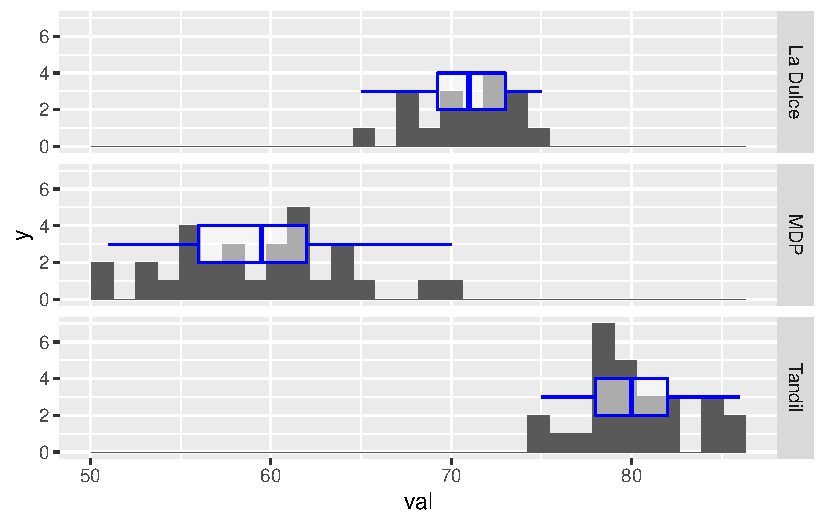
\includegraphics{curasem_files/figure-pdf/unnamed-chunk-10-1.pdf}

\hypertarget{anuxe1lisis-conjunto-de-6-tratamientos-1}{%
\subsubsection{Análisis conjunto de 6
tratamientos}\label{anuxe1lisis-conjunto-de-6-tratamientos-1}}

\begin{verbatim}
                                    sitio La Dulce MDP Tandil
cultivo prod                                                 
Trigo   RANCONA_TRIO_300                         3   3      3
        RIZODERMA                                3   3      3
        RIZODERMA + VITAGROW + STZN              3   3      3
        SISTIVA_PREMIS                           3   3      3
        SISTIVA_PREMIS + ALZ_12051               3   3      3
        VIBRANCE_INTEGRAL                        3   3      3
\end{verbatim}

\begin{longtable}[]{@{}lrrr@{}}
\toprule()
& Chisq & Df & Pr(\textgreater Chisq) \\
\midrule()
\endhead
prod & 2.913131 & 5 & 0.7133764 \\
\bottomrule()
\end{longtable}

\begin{longtable}[]{@{}
  >{\raggedright\arraybackslash}p{(\columnwidth - 14\tabcolsep) * \real{0.0366}}
  >{\raggedright\arraybackslash}p{(\columnwidth - 14\tabcolsep) * \real{0.3415}}
  >{\raggedleft\arraybackslash}p{(\columnwidth - 14\tabcolsep) * \real{0.1098}}
  >{\raggedleft\arraybackslash}p{(\columnwidth - 14\tabcolsep) * \real{0.1098}}
  >{\raggedleft\arraybackslash}p{(\columnwidth - 14\tabcolsep) * \real{0.0976}}
  >{\raggedleft\arraybackslash}p{(\columnwidth - 14\tabcolsep) * \real{0.1098}}
  >{\raggedleft\arraybackslash}p{(\columnwidth - 14\tabcolsep) * \real{0.1098}}
  >{\raggedright\arraybackslash}p{(\columnwidth - 14\tabcolsep) * \real{0.0854}}@{}}
\toprule()
\begin{minipage}[b]{\linewidth}\raggedright
\end{minipage} & \begin{minipage}[b]{\linewidth}\raggedright
prod
\end{minipage} & \begin{minipage}[b]{\linewidth}\raggedleft
response
\end{minipage} & \begin{minipage}[b]{\linewidth}\raggedleft
SE
\end{minipage} & \begin{minipage}[b]{\linewidth}\raggedleft
df
\end{minipage} & \begin{minipage}[b]{\linewidth}\raggedleft
lower.CL
\end{minipage} & \begin{minipage}[b]{\linewidth}\raggedleft
upper.CL
\end{minipage} & \begin{minipage}[b]{\linewidth}\raggedright
.group
\end{minipage} \\
\midrule()
\endhead
1 & RIZODERMA & 71.92191 & 6.064280 & 2.16599 & 45.69791 & 91.90712 &
a \\
6 & SISTIVA\_PREMIS + ALZ\_12051 & 71.74619 & 6.075791 & 2.16599 &
45.50335 & 91.80026 & a \\
3 & SISTIVA\_PREMIS & 70.28021 & 6.167430 & 2.16599 & 43.89683 &
90.89203 & a \\
4 & RIZODERMA + VITAGROW + STZN & 70.02282 & 6.182726 & 2.16599 &
43.61779 & 90.72954 & a \\
5 & VIBRANCE\_INTEGRAL & 69.88967 & 6.190548 & 2.16599 & 43.47378 &
90.64513 & a \\
2 & RANCONA\_TRIO\_300 & 69.52689 & 6.211545 & 2.16599 & 43.08263 &
90.41397 & a \\
\bottomrule()
\end{longtable}

\hypertarget{anuxe1lisis-conjunto-de-mdp-tandil-1}{%
\subsubsection{Análisis conjunto de MDP +
Tandil}\label{anuxe1lisis-conjunto-de-mdp-tandil-1}}

\begin{verbatim}
                                    sitio MDP Tandil
cultivo prod                                        
Trigo   CHECK                               3      3
        CURACYT                             3      3
        RANCONA_TRIO_300                    3      3
        RIZODERMA                           3      3
        RIZODERMA + VITAGROW + STZN         3      3
        SISTIVA_PREMIS                      3      3
        SISTIVA_PREMIS + ALLTEC_ZN          3      3
        SISTIVA_PREMIS + ALZ_12051          3      3
        VIBRANCE_INTEGRAL                   3      3
\end{verbatim}

\begin{longtable}[]{@{}lrrr@{}}
\toprule()
& Chisq & Df & Pr(\textgreater Chisq) \\
\midrule()
\endhead
prod & 0.5246373 & 8 & 0.9998399 \\
\bottomrule()
\end{longtable}

\begin{longtable}[]{@{}
  >{\raggedright\arraybackslash}p{(\columnwidth - 14\tabcolsep) * \real{0.0361}}
  >{\raggedright\arraybackslash}p{(\columnwidth - 14\tabcolsep) * \real{0.3373}}
  >{\raggedleft\arraybackslash}p{(\columnwidth - 14\tabcolsep) * \real{0.1084}}
  >{\raggedleft\arraybackslash}p{(\columnwidth - 14\tabcolsep) * \real{0.1084}}
  >{\raggedleft\arraybackslash}p{(\columnwidth - 14\tabcolsep) * \real{0.1084}}
  >{\raggedleft\arraybackslash}p{(\columnwidth - 14\tabcolsep) * \real{0.1084}}
  >{\raggedleft\arraybackslash}p{(\columnwidth - 14\tabcolsep) * \real{0.1084}}
  >{\raggedright\arraybackslash}p{(\columnwidth - 14\tabcolsep) * \real{0.0843}}@{}}
\toprule()
\begin{minipage}[b]{\linewidth}\raggedright
\end{minipage} & \begin{minipage}[b]{\linewidth}\raggedright
prod
\end{minipage} & \begin{minipage}[b]{\linewidth}\raggedleft
response
\end{minipage} & \begin{minipage}[b]{\linewidth}\raggedleft
SE
\end{minipage} & \begin{minipage}[b]{\linewidth}\raggedleft
df
\end{minipage} & \begin{minipage}[b]{\linewidth}\raggedleft
lower.CL
\end{minipage} & \begin{minipage}[b]{\linewidth}\raggedleft
upper.CL
\end{minipage} & \begin{minipage}[b]{\linewidth}\raggedright
.group
\end{minipage} \\
\midrule()
\endhead
9 & RIZODERMA & 71.03603 & 10.54155 & 1.055672 & 0 & 100 & a \\
6 & CURACYT & 70.99991 & 10.54544 & 1.055672 & 0 & 100 & a \\
3 & SISTIVA\_PREMIS + ALZ\_12051 & 70.94149 & 10.55171 & 1.055672 & 0 &
100 & a \\
5 & CHECK & 70.56185 & 10.59196 & 1.055672 & 0 & 100 & a \\
7 & SISTIVA\_PREMIS + ALLTEC\_ZN & 70.37117 & 10.61184 & 1.055672 & 0 &
100 & a \\
1 & RIZODERMA + VITAGROW + STZN & 70.15986 & 10.63362 & 1.055672 & 0 &
100 & a \\
8 & RANCONA\_TRIO\_300 & 70.11556 & 10.63815 & 1.055672 & 0 & 100 & a \\
2 & SISTIVA\_PREMIS & 69.91311 & 10.65870 & 1.055672 & 0 & 100 & a \\
4 & VIBRANCE\_INTEGRAL & 69.82981 & 10.66708 & 1.055672 & 0 & 100 & a \\
\bottomrule()
\end{longtable}

\hypertarget{rinde}{%
\section{Rinde}\label{rinde}}

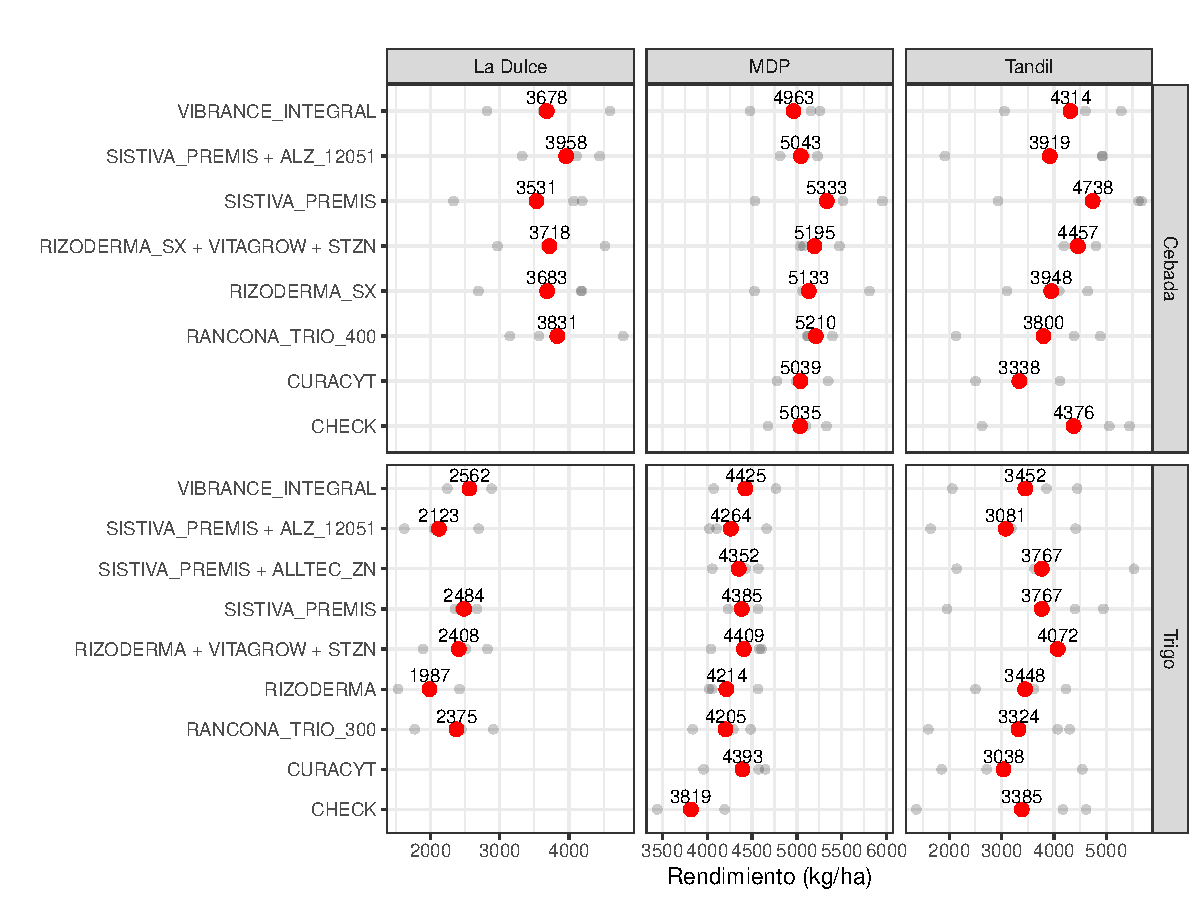
\includegraphics{curasem_files/figure-pdf/unnamed-chunk-17-1.pdf}

\hypertarget{cebada-1}{%
\subsection{Cebada}\label{cebada-1}}

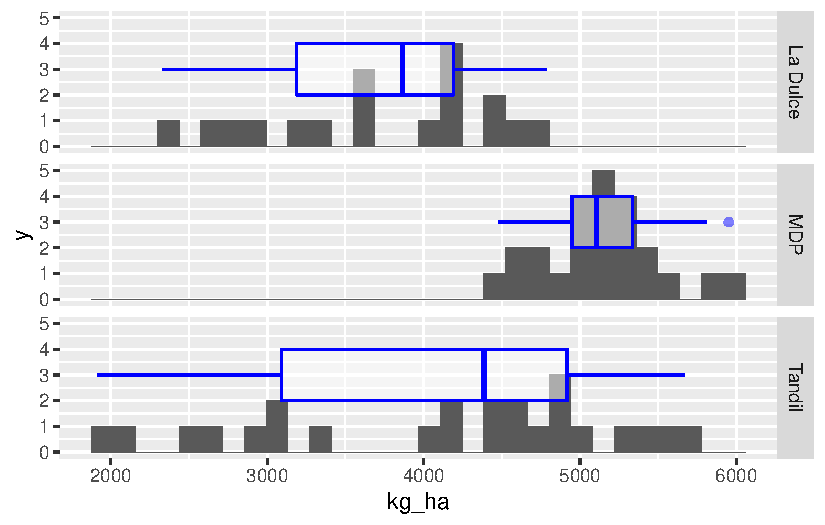
\includegraphics{curasem_files/figure-pdf/unnamed-chunk-19-1.pdf}

\hypertarget{anuxe1lisis-individual-intra-sitio}{%
\subsubsection{Análisis individual
intra-sitio}\label{anuxe1lisis-individual-intra-sitio}}

\begin{longtable}[]{@{}lr@{}}
\toprule()
sitio & cv\% \\
\midrule()
\endhead
La Dulce & 21.543114 \\
MDP & 7.986728 \\
Tandil & 30.562219 \\
\bottomrule()
\end{longtable}

\begin{verbatim}
# A tibble: 22 x 6
# Groups:   sitio [3]
   sitio    prod                           kg_ha conf.low conf.high .group
   <chr>    <fct>                          <dbl>    <dbl>     <dbl> <fct> 
 1 La Dulce SISTIVA_PREMIS + ALZ_12051     3958.    2888.     5029. " a"  
 2 La Dulce RANCONA_TRIO_400               3831.    2761.     4902. " a"  
 3 La Dulce RIZODERMA_SX + VITAGROW + STZN 3718.    2648.     4789. " a"  
 4 La Dulce RIZODERMA_SX                   3683.    2613.     4754. " a"  
 5 La Dulce VIBRANCE_INTEGRAL              3678.    2608.     4748. " a"  
 6 La Dulce SISTIVA_PREMIS                 3531.    2460.     4601. " a"  
 7 MDP      SISTIVA_PREMIS                 5333.    4812.     5854. " a"  
 8 MDP      RANCONA_TRIO_400               5210.    4689.     5731. " a"  
 9 MDP      RIZODERMA_SX + VITAGROW + STZN 5195.    4674.     5716. " a"  
10 MDP      RIZODERMA_SX                   5133.    4612.     5653. " a"  
11 MDP      SISTIVA_PREMIS + ALZ_12051     5043.    4523.     5564. " a"  
12 MDP      CURACYT                        5039.    4519.     5560. " a"  
13 MDP      CHECK                          5035.    4514.     5556. " a"  
14 MDP      VIBRANCE_INTEGRAL              4963.    4442.     5483. " a"  
15 Tandil   SISTIVA_PREMIS                 4738     3201.     6275. " a"  
16 Tandil   RIZODERMA_SX + VITAGROW + STZN 4457.    2920.     5995. " a"  
17 Tandil   CHECK                          4376.    2839.     5914. " a"  
18 Tandil   VIBRANCE_INTEGRAL              4314.    2777.     5852. " a"  
19 Tandil   RIZODERMA_SX                   3948.    2410.     5485. " a"  
20 Tandil   SISTIVA_PREMIS + ALZ_12051     3919     2382.     5456. " a"  
21 Tandil   RANCONA_TRIO_400               3800.    2263.     5338. " a"  
22 Tandil   CURACYT                        3338     1801.     4875. " a"  
\end{verbatim}

\hypertarget{anuxe1lisis-conjunto-de-6-tratamientos-2}{%
\subsubsection{Análisis conjunto de 6
tratamientos}\label{anuxe1lisis-conjunto-de-6-tratamientos-2}}

\begin{verbatim}
                                       sitio La Dulce MDP Tandil
cultivo prod                                                    
cebada  RANCONA_TRIO_400                            3   3      3
        RIZODERMA_SX                                3   3      3
        RIZODERMA_SX + VITAGROW + STZN              3   3      3
        SISTIVA_PREMIS                              3   3      3
        SISTIVA_PREMIS + ALZ_12051                  3   3      3
        VIBRANCE_INTEGRAL                           3   3      3
\end{verbatim}

\begin{longtable}[]{@{}
  >{\raggedright\arraybackslash}p{(\columnwidth - 8\tabcolsep) * \real{0.4493}}
  >{\raggedleft\arraybackslash}p{(\columnwidth - 8\tabcolsep) * \real{0.1304}}
  >{\raggedleft\arraybackslash}p{(\columnwidth - 8\tabcolsep) * \real{0.1304}}
  >{\raggedleft\arraybackslash}p{(\columnwidth - 8\tabcolsep) * \real{0.1449}}
  >{\raggedright\arraybackslash}p{(\columnwidth - 8\tabcolsep) * \real{0.1449}}@{}}
\toprule()
\begin{minipage}[b]{\linewidth}\raggedright
prod
\end{minipage} & \begin{minipage}[b]{\linewidth}\raggedleft
kg\_ha
\end{minipage} & \begin{minipage}[b]{\linewidth}\raggedleft
conf.low
\end{minipage} & \begin{minipage}[b]{\linewidth}\raggedleft
conf.high
\end{minipage} & \begin{minipage}[b]{\linewidth}\raggedright
tukey\_10\%
\end{minipage} \\
\midrule()
\endhead
SISTIVA\_PREMIS & 4442.936 & 3125.399 & 5991.600 & a \\
RIZODERMA\_SX + VITAGROW + STZN & 4424.593 & 3110.018 & 5970.296 & a \\
VIBRANCE\_INTEGRAL & 4269.422 & 2980.149 & 5789.824 & a \\
SISTIVA\_PREMIS + ALZ\_12051 & 4231.966 & 2948.869 & 5746.192 & a \\
RANCONA\_TRIO\_400 & 4207.057 & 2928.082 & 5717.161 & a \\
RIZODERMA\_SX & 4205.807 & 2927.039 & 5715.703 & a \\
\bottomrule()
\end{longtable}

\hypertarget{anuxe1lisis-conjunto-de-mdp-tandil-2}{%
\subsubsection{Análisis conjunto de MDP +
Tandil}\label{anuxe1lisis-conjunto-de-mdp-tandil-2}}

\begin{verbatim}
                                       sitio MDP Tandil
cultivo prod                                           
cebada  CHECK                                  3      3
        CURACYT                                3      3
        RANCONA_TRIO_400                       3      3
        RIZODERMA_SX                           3      3
        RIZODERMA_SX + VITAGROW + STZN         3      3
        SISTIVA_PREMIS                         3      3
        SISTIVA_PREMIS + ALZ_12051             3      3
        VIBRANCE_INTEGRAL                      3      3
\end{verbatim}

\begin{longtable}[]{@{}
  >{\raggedright\arraybackslash}p{(\columnwidth - 8\tabcolsep) * \real{0.4493}}
  >{\raggedleft\arraybackslash}p{(\columnwidth - 8\tabcolsep) * \real{0.1304}}
  >{\raggedleft\arraybackslash}p{(\columnwidth - 8\tabcolsep) * \real{0.1304}}
  >{\raggedleft\arraybackslash}p{(\columnwidth - 8\tabcolsep) * \real{0.1449}}
  >{\raggedright\arraybackslash}p{(\columnwidth - 8\tabcolsep) * \real{0.1449}}@{}}
\toprule()
\begin{minipage}[b]{\linewidth}\raggedright
prod
\end{minipage} & \begin{minipage}[b]{\linewidth}\raggedleft
kg\_ha
\end{minipage} & \begin{minipage}[b]{\linewidth}\raggedleft
conf.low
\end{minipage} & \begin{minipage}[b]{\linewidth}\raggedleft
conf.high
\end{minipage} & \begin{minipage}[b]{\linewidth}\raggedright
tukey\_10\%
\end{minipage} \\
\midrule()
\endhead
SISTIVA\_PREMIS & 5035.340 & 2509.509 & 7561.171 & a \\
RIZODERMA\_SX + VITAGROW + STZN & 4826.075 & 2300.244 & 7351.906 & a \\
CHECK & 4705.766 & 2179.935 & 7231.597 & a \\
VIBRANCE\_INTEGRAL & 4638.489 & 2112.658 & 7164.320 & a \\
RIZODERMA\_SX & 4540.147 & 2014.316 & 7065.978 & a \\
RANCONA\_TRIO\_400 & 4505.330 & 1979.499 & 7031.161 & a \\
SISTIVA\_PREMIS + ALZ\_12051 & 4481.245 & 1955.414 & 7007.076 & a \\
CURACYT & 4188.672 & 1662.841 & 6714.503 & a \\
\bottomrule()
\end{longtable}

\hypertarget{trigo-1}{%
\subsection{Trigo}\label{trigo-1}}

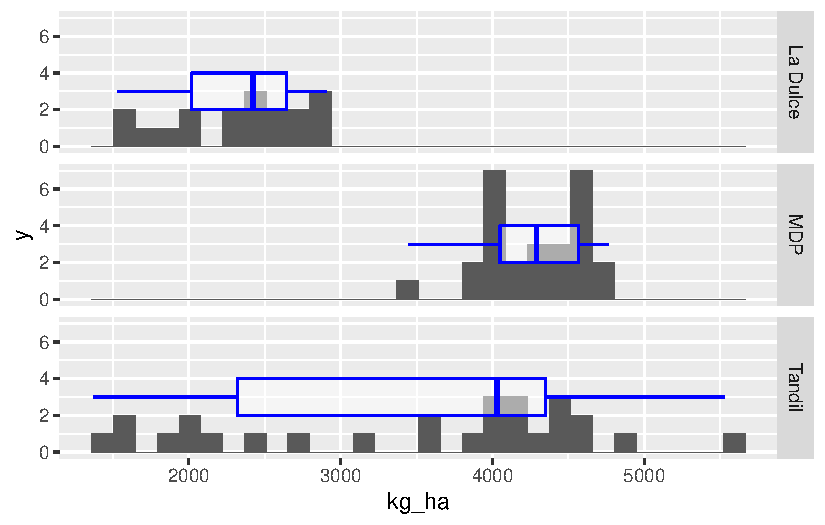
\includegraphics{curasem_files/figure-pdf/unnamed-chunk-24-1.pdf}

\hypertarget{anuxe1lisis-individual-intra-sitio-1}{%
\subsubsection{Análisis individual
intra-sitio}\label{anuxe1lisis-individual-intra-sitio-1}}

\begin{longtable}[]{@{}lr@{}}
\toprule()
sitio & cv\% \\
\midrule()
\endhead
La Dulce & 19.821780 \\
MDP & 7.005211 \\
Tandil & 40.378135 \\
\bottomrule()
\end{longtable}

\begin{verbatim}
# A tibble: 24 x 6
# Groups:   sitio [3]
   sitio    prod                        kg_ha conf.low conf.high .group
   <chr>    <fct>                       <dbl>    <dbl>     <dbl> <fct> 
 1 La Dulce VIBRANCE_INTEGRAL           2562.    2006.     3119. " a"  
 2 La Dulce SISTIVA_PREMIS              2484.    1927.     3041. " a"  
 3 La Dulce RIZODERMA + VITAGROW + STZN 2408.    1852.     2965. " a"  
 4 La Dulce RANCONA_TRIO_300            2375.    1818.     2932. " a"  
 5 La Dulce SISTIVA_PREMIS + ALZ_12051  2123.    1566.     2680. " a"  
 6 La Dulce RIZODERMA                   1987.    1430.     2544. " a"  
 7 MDP      VIBRANCE_INTEGRAL           4425.    4034.     4817. " a"  
 8 MDP      RIZODERMA + VITAGROW + STZN 4409.    4018.     4801. " a"  
 9 MDP      CURACYT                     4393.    4001.     4785. " a"  
10 MDP      SISTIVA_PREMIS              4385.    3993.     4777. " a"  
11 MDP      SISTIVA_PREMIS + ALLTEC_ZN  4352.    3960.     4743. " a"  
12 MDP      SISTIVA_PREMIS + ALZ_12051  4264.    3872.     4656. " a"  
13 MDP      RIZODERMA                   4214.    3822.     4605. " a"  
14 MDP      RANCONA_TRIO_300            4205.    3813.     4597. " a"  
15 MDP      CHECK                       3819.    3427.     4211. " a"  
16 Tandil   RIZODERMA + VITAGROW + STZN 4072.    2411.     5732. " a"  
17 Tandil   SISTIVA_PREMIS + ALLTEC_ZN  3767     2106.     5428. " a"  
18 Tandil   SISTIVA_PREMIS              3767.    2106.     5427. " a"  
19 Tandil   VIBRANCE_INTEGRAL           3452.    1792.     5113. " a"  
20 Tandil   RIZODERMA                   3448.    1787.     5108. " a"  
21 Tandil   CHECK                       3385.    1725.     5046. " a"  
22 Tandil   RANCONA_TRIO_300            3324.    1663.     4984. " a"  
23 Tandil   SISTIVA_PREMIS + ALZ_12051  3081     1420.     4742. " a"  
24 Tandil   CURACYT                     3038     1377.     4699. " a"  
\end{verbatim}

\hypertarget{anuxe1lisis-conjunto-de-6-tratamientos-3}{%
\subsubsection{Análisis conjunto de 6
tratamientos}\label{anuxe1lisis-conjunto-de-6-tratamientos-3}}

\begin{verbatim}
                                    sitio La Dulce MDP Tandil
cultivo prod                                                 
trigo   RANCONA_TRIO_300                         3   3      3
        RIZODERMA                                3   3      3
        RIZODERMA + VITAGROW + STZN              3   3      3
        SISTIVA_PREMIS                           3   3      3
        SISTIVA_PREMIS + ALZ_12051               3   3      3
        VIBRANCE_INTEGRAL                        3   3      3
\end{verbatim}

\begin{longtable}[]{@{}
  >{\raggedright\arraybackslash}p{(\columnwidth - 8\tabcolsep) * \real{0.4179}}
  >{\raggedleft\arraybackslash}p{(\columnwidth - 8\tabcolsep) * \real{0.1343}}
  >{\raggedleft\arraybackslash}p{(\columnwidth - 8\tabcolsep) * \real{0.1493}}
  >{\raggedleft\arraybackslash}p{(\columnwidth - 8\tabcolsep) * \real{0.1493}}
  >{\raggedright\arraybackslash}p{(\columnwidth - 8\tabcolsep) * \real{0.1493}}@{}}
\toprule()
\begin{minipage}[b]{\linewidth}\raggedright
prod
\end{minipage} & \begin{minipage}[b]{\linewidth}\raggedleft
kg\_ha
\end{minipage} & \begin{minipage}[b]{\linewidth}\raggedleft
conf.low
\end{minipage} & \begin{minipage}[b]{\linewidth}\raggedleft
conf.high
\end{minipage} & \begin{minipage}[b]{\linewidth}\raggedright
tukey\_10\%
\end{minipage} \\
\midrule()
\endhead
RIZODERMA + VITAGROW + STZN & 3629.795 & 1444.6578 & 5814.932 & a \\
SISTIVA\_PREMIS & 3545.268 & 1360.1303 & 5730.405 & a \\
VIBRANCE\_INTEGRAL & 3480.071 & 1294.9337 & 5665.208 & a \\
RANCONA\_TRIO\_300 & 3301.149 & 1116.0119 & 5486.287 & a \\
RIZODERMA & 3216.052 & 1030.9148 & 5401.189 & a \\
SISTIVA\_PREMIS + ALZ\_12051 & 3155.960 & 970.8229 & 5341.098 & a \\
\bottomrule()
\end{longtable}

\hypertarget{anuxe1lisis-conjunto-de-mdp-tandil-3}{%
\subsubsection{Análisis conjunto de MDP +
Tandil}\label{anuxe1lisis-conjunto-de-mdp-tandil-3}}

\begin{verbatim}
                                    sitio MDP Tandil
cultivo prod                                        
trigo   CHECK                               3      3
        CURACYT                             3      3
        RANCONA_TRIO_300                    3      3
        RIZODERMA                           3      3
        RIZODERMA + VITAGROW + STZN         3      3
        SISTIVA_PREMIS                      3      3
        SISTIVA_PREMIS + ALLTEC_ZN          3      3
        SISTIVA_PREMIS + ALZ_12051          3      3
        VIBRANCE_INTEGRAL                   3      3
\end{verbatim}

\begin{longtable}[]{@{}lrrrl@{}}
\toprule()
prod & kg\_ha & conf.low & conf.high & tukey\_10\% \\
\midrule()
\endhead
RIZODERMA + VITAGROW + STZN & 4240.460 & 2600.406 & 5880.514 & a \\
SISTIVA\_PREMIS & 4075.861 & 2435.807 & 5715.915 & a \\
SISTIVA\_PREMIS + ALLTEC\_ZN & 4059.334 & 2419.280 & 5699.388 & a \\
VIBRANCE\_INTEGRAL & 3938.859 & 2298.805 & 5578.913 & a \\
RIZODERMA & 3830.709 & 2190.655 & 5470.763 & a \\
RANCONA\_TRIO\_300 & 3764.294 & 2124.240 & 5404.348 & a \\
CURACYT & 3715.561 & 2075.507 & 5355.615 & a \\
SISTIVA\_PREMIS + ALZ\_12051 & 3672.535 & 2032.481 & 5312.589 & a \\
CHECK & 3602.204 & 1962.150 & 5242.258 & a \\
\bottomrule()
\end{longtable}



\end{document}
